\documentclass[titlepage]{article}
\usepackage[english]{babel}
\usepackage[utf8]{inputenc}
\usepackage[T1]{fontenc}
\usepackage{lmodern}
\usepackage{textcomp}
\usepackage{amsmath}
\usepackage{amssymb}
\usepackage{listings}
\usepackage{graphicx}
\usepackage{float}
\usepackage{comment}
\excludecomment{toex}
\usepackage{fullpage}
\usepackage{blkarray}
\usepackage[usenames,dvipsnames]{xcolor}
\usepackage[export]{adjustbox}
\definecolor{bg}{HTML}{FFFFEE}
\lstset{language=Scala,backgroundcolor=\color{bg},frame=single,showspaces=false,basicstyle=\ttfamily,literate={"}{\textquotedbl}1,literate={'}{\textquotesingle}1,keywordstyle=\color{NavyBlue}, breaklines=true,showstringspaces=false,commentstyle=\footnotesize\color{Turquoise},rulecolor=\color{black},otherkeywords={colorbar},literate=%
                {é}{{\'e}}{1}%
                {è}{{\`e}}{1}%
                {à}{{\`a}}{1}%
                {ç}{{\c{c}}}{1}%
                {œ}{{\oe}}{1}%
                {ù}{{\`u}}{1}%
                {É}{{\'E}}{1}%
                {È}{{\`E}}{1}%
                {À}{{\`A}}{1}%
                {Ç}{{\c{C}}}{1}%
                {Œ}{{\OE}}{1}%
                {Ê}{{\^E}}{1}%
                {ê}{{\^e}}{1}%
                {î}{{\^i}}{1}%
                {ô}{{\^o}}{1}%
                {û}{{\^u}}{1}%
                {ë}{{\¨{e}}}1
                {û}{{\^{u}}}1
                {â}{{\^{a}}}1
                {Â}{{\^{A}}}1
                {Î}{{\^{I}}}1}

\usepackage{hyperref}
\hypersetup{colorlinks=false,
citecolor=black,
filecolor=black,
linkcolor=black,
urlcolor=black, 
linkbordercolor={1 0.5 0}}
\setcounter{MaxMatrixCols}{20}
\usepackage{titlesec}
\titleclass{\subsubsubsection}{straight}[\subsection]

\newcounter{subsubsubsection}[subsubsection]
\renewcommand\thesubsubsubsection{\thesubsubsection.\arabic{subsubsubsection}}

\titleformat{\subsubsubsection}
  {\normalfont\normalsize\bfseries}{\thesubsubsubsection}{1em}{}
\titlespacing*{\subsubsubsection}
{0pt}{3.25ex plus 1ex minus .2ex}{1.5ex plus .2ex}
\makeatletter
\def\toclevel@subsubsubsection{4}
\def\l@subsubsubsection{\@dottedtocline{4}{7em}{4em}}
\makeatother
\setcounter{secnumdepth}{4}
\setcounter{tocdepth}{4}
\newcommand{\HRule}{\rule{\linewidth}{0.5mm}}
\definecolor{RoyalRed}{RGB}{157,16, 45}
\titleformat{\section}
{\normalfont\LARGE\sffamily\bfseries}{\underline{Section \thesection :}}{1em}{}

\begin{document}

\title{TX - Parallel Programming: Distributing the Hodgkin-Huxley Model}
\date{P17}
\author{Anton Ippolitov, GI04}
\maketitle

\tableofcontents
\newpage

\section{Introduction and description of the model}
This project has been conducted during the spring semester at the Universit\'e de Technologie de Compi\`egne under the supervision of Dr. Tien Tuan Dao. It consisted in design and implementation of an agent-based distributed model of human gait. The model consists of two agent-based subsystems corresponding to the soleus muscle and the tibialis anterior muscle. Each subsystem is composed of a number of motor unit agents (150 for tibialis anterior and 458 for soleus). There is also a decision subsystem which orchestrates the flow of the simulation. At every tick of the simulation, a certain percentage of motor units in each subsystem is activated and calculates its membrane potential (using the equations from the Hodkgin-Huxley model). The potentials of all active motor units are then summed and are sent to the decision subsystem. The percentages of active motor units in every subsystem at each tick are determined by the percent gait cycle values that are given in the model. 
\\\\
The goal was to create a scalable robust implementation of this model that can be distributed across multiple machines.
\section{Choice of technology}
The first stage was to choose the most suitable technology for the model implementation. There are a lot of libraries and frameworks for distributed computing but they mostly fall into two broad categories: data-parallel and task-parallel. The difference is in the nature of the operations: data parallelism means that same operations are performed on different subsets of same data while task parallelism is more flexible and allows parallel operations that can be different and can be performed on same or different data. Thus, the data-parallel computations can be synchronous while task-parallel computations are asynchronous. The benefits of a data-parallel approach are the ease of load balancing and potentially higher speed-up whereas the task-parallel approach is more flexible. In our case, the requirements for the model were the following:
\begin{itemize}
\item Be able to distribute and manage tasks that can be potentially heterogeneous. 
\item Tasks should be easily synchronizable and processes/threads executing them have to be able to easily communicate with each other. 
\item The distribution should be handled not only across different cores but also across a cluster of machines (nodes).
\item The framework should be fast and be able to handle heavy calculations.
\end{itemize}
These requirements correspond more to a task-parallel framework than a data-parallel one. There were several technologies that were considered:
\begin{itemize}
\item \textbf{MPI (Message Passing Interface)} - MPI is a "a standardized means of exchanging messages between multiple computers running a parallel program across distributed memory". MPI is a standard for writing distributed applications. There are several implementations of this standard, most notably in C\texttt{++} and Fortran. MPI fulfils the aforementioned criteria and there is a lot of available documentation (though most of it is old or poorly structured).
\item \textbf{OpenMP} - OpenMP is "a specification for a set of compiler directives, library routines, and environment variables that can be used to specify high-level parallelism in Fortran and C/C++ programs". The problem with OpenMP is that it is hard to use it in a cluster of machines: "As of 2017 [OpenMP] only runs efficiently in shared-memory multiprocessor platforms".
\item \textbf{Charm\texttt{++}} - Charm\texttt{++} is a language based on C\texttt{++} used for creating distributed applications. It is similar to MPI but is harder to use for expressing global control flow, global communication and concurrency management. It also has fewer libraries. Its advantages are load balancing and fault-tolerance that are not priorities for this project. 
\item \textbf{RaftLib} - RaftLib is a C\texttt{++} library for creating task- and data-parallel distributed programs. At the moment of writing, it is still in an alpha stage so it is not completely robust and does not a have a large community or extensive documentation. It is also not clear if the library can function in a distributed-memory setting (i.e. in a cluster of machines). 
\item \textbf{Intel TBB (Threading Building Blocks)} - TBB is a C\texttt{++} library for writing data- and task-parallel programs. However, it can not be used in a cluster either.
\item \textbf{Akka} - Akka is a Java/Scala or C\#/F\# toolkit used for creating scalable and distributed applications. It is based on the actor model: the application is designed as a system of actors (objects which encapsulate state and behavior) that communicate with each other using messages. Akka fulfils all the criteria listed above, is robust, has an extensive documentation and an active community.  
\item \textbf{CAF (C\texttt{++} Actor Framework)} - CAF is a framework similar to Akka but is more recent so it is less complete and robust (version 0.15 at the moment of writing) with a much smaller community.
\item \textbf{Apache Spark} - Spark is a framework for distributed computing allowing for fast in-memory data-processing. It is written in Scala but can be used has a Java, Scala, Python and R APIs. It is perfect for data-parallel computing on large quantities of data but is not suitable for task-parallel computations.
\end{itemize}

In conclusion, Akka seemed to be the most suitable technology for this project. There is a .NET and a Java/Scala version so I have chosen Scala as I was the most familiar with it. It is also much more powerful and concise than Java as it is a functional and an object-oriented language whereas Java is not functional (Java 8 has new functional features but Scala is still much more advanced and flexible). 

\section{Implementing the model}
\subsection{Back-end: Akka}
\subsubsection{Creating the actors}
The entities in the model can easily be represented using the conventions from the actor model. A motor system (motor pool) can be an actor that manages child motor unit actors. There should also be one master actor that coordinates the flow of the simulation. The three actor classes, Master, MotorSystem and MotorUnit will do the following:
\begin{itemize}
\item \textbf{Master} - The Master will be a singleton actor. Its fields are the total number of ticks that the simulation will run for and the number of motor systems that it will manage. When the Master starts, it waits until all MotorSystem actors send it registration messages, meaning that they are up and ready to start the simulation. When all MotorSystem actors are ready, the master starts the simulation. It sends a \textit{ProcessTick} message to all MotorSystem actors telling them to start the tick calculations. It then waits until all MotorSystems finish their calculations and send it the \textit{ResultSum} message containing the result of the tick calculation. When all results are received, the Master continues with the next tick by sending a new \textit{ProcessTick} message. After processing the final tick, the Master sends a message to MotorSystems telling them to shut down and the shuts down itself.
\item \textbf{MotorSystem} - There can be one or several MotorSystem actors. In our model there are two of them, corresponding to Tibialis Anteior and Soleus. The MotorSystems are created with parameters specifying the number of their child MotorUnits as well as the percent gait cycle values. When a MotorSystem is created, it instantiates all child MotorUnits actors and then sends a registration message to the Master actor saying that it is ready. It then waits for \textit{ProcessTick} messages from the Master. When it receives one, it sends a \textit{Caclulate} message to a certain number of MotorUnit actors that are supposed to be active according to the percent gait cycle. All \textit{Calculate} messages contain parameters for performing the calculation of the membrane potential of the motor unit. The MotorSystem then waits for \textit{Result} messages from its child MotorUnits containing the voltage time series. When it receives a \textit{Result} message, it sums the values of the received time series with all the other ones. When all messages from all MotorUnits are received, the MotorSystem sends the final sum in a \textit{ResultSum} message to the Master, signifying that the system has finished its tick calculations. It is now ready to receive the next \textit{ProcessTick} message.
\item \textbf{MotorUnit} - MotorUnit actors are instantiated by MotorSystem actors. MotorUnit's only role is to receive \textit{Caclulate} messages from its parent MotorSystem, calculate the membrane potential using parameters specified in the message and then send a \textit{Result} message to the sender. The calculation is explained in detail in the \hyperref[sec:calc]{last part} of this section.
\end{itemize}
All actors can be on the same node (Akka will make sure that they will use all available cores) or can be distributed across a cluster. The ideal situation for simulations with a large number of MotorUnits is to have a dedicated node for each MotorSystem as well as for the Master. The figure \ref{fig:architecture} illustrates this architecture.
\begin{figure}[H]
  \hspace*{-2cm}
  \includegraphics[scale=0.19]{architecture.png}
  \caption{Architecture of the distributed model using Akka}
  \label{fig:architecture}
\end{figure}
In the figure, there are two MotorSystems each one having a dedicated node. The Master also has a dedicated node. In this illustration, the Master actor is instantiated using the Play framework, this is explained in detail in the \hyperref[sec:front]{front-end subsection}. 
\subsubsection{Digitizing the percent gait cycle graphs}
The values for the percent gait potential of Tibialis Anterior and Soleus were only available as graphs with no explicitly defined functions, nor numerical values. 
\begin{figure}[H]
  \centering
	\includegraphics[scale=0.4]{graphs.png}
	\caption{Percent gait cycle graphs}
  \label{fig:graphs}
\end{figure}
In order to extract the numerical values from graphs, graph digitizing software can be used. There is a number of different tools available and I have opted for WebPlotDigitizer for its convenience as it can be used directly in a browser. The first step is to mark the axes on the picture and then to place points on the plot that follow the function line, as shown in the figure~\ref{fig:dig}. The $(x, y)$ tuples generated this way can then be exported in .csv format.
\begin{figure}[H]
  \centering
	\includegraphics[scale=0.4]{dig.png}
	\caption{Using WebPlotDigitizer to extract numerical data from the Tibialis Anterior percent gait cycle graph}
  \label{fig:dig}
\end{figure}
As the points were placed manually on the graph, they were not evenly distributed. In order to distribute them evenly it is possible to use interpolation functions in MATLAB. Here is a code snippet that will generate a list of y values for each integer x from 0 to 100 using the Tibialis Anterior dataset:
\begin{lstlisting}[language=MATLAB]
name = 'TibialisInitialDataset.csv';
M = csvread(name); %read data exported from WebPlotDigitizer
x = M(:, 1);
v = M(:, 2);
xq = 0:100; %query points
yq = interp1(x, v, xq); %interpolate
csvwrite('TibialisInterpolatedDataset.csv', yq);
\end{lstlisting}
We have chosen a step of 1 for x values as we want the simulation to last 101 ticks. Here are the resulting datasets:
\begin{figure}[H]
  \centering
	\includegraphics[scale=0.6]{int1.png}
	\caption{Numerical values for the Soleus percent gait cycle with step = 1 for x}
  \label{fig:int1}
\end{figure}
\begin{figure}[H]
  \centering
	\includegraphics[scale=0.6]{int2.png}
	\caption{Numerical values for the Tibialis Anterior percent gait cycle with step = 1 for x}
  \label{fig:int2}
\end{figure}
These values can now be used by the MotorSystem actors to determine the percentage of active MotorUnits at each tick.
\subsubsection{Membrane potential calculation}
\label{sec:calc}
The calculation performed by each of the MotorUnit actors is based on the Hodkin-Huxley model. Here is a MATLAB version of the model:
\begin{lstlisting}[language=MATLAB]
function [V,m,h,n,t] = Potential(I, tspan, v, mi, hi, ni)   

  dt = 0.001;               % time step for forward euler method
  loop  = ceil(tspan/dt);   % no. of iterations of euler
  
  gNa = 120;  
  eNa = 115;
  gK = 36;  
  eK = -12;
  gL = 0.3;  
  eL = 10.6;
 
  % Initializing variable vectors
  t = (1:loop)*dt;
  V = zeros(loop,1);
  m = zeros(loop,1);
  h = zeros(loop,1);
  n = zeros(loop,1);

  % Set initial values for the variables
  V(1) = v;
  m(1) = mi;
  h(1) = hi;
  n(1) = ni;
   
  for i=1:loop-1 
      V(i+1) = V(i) + dt*(gNa*m(i)^3*h(i)*(eNa-(V(i)+65)) + gK*n(i)^4*(eK-(V(i)+65)) + gL*(eL-(V(i)+65)) + I);
      m(i+1) = m(i) + dt*(alphaM(V(i))*(1-m(i)) - betaM(V(i))*m(i));
      h(i+1) = h(i) + dt*(alphaH(V(i))*(1-h(i)) - betaH(V(i))*h(i));
      n(i+1) = n(i) + dt*(alphaN(V(i))*(1-n(i)) - betaN(V(i))*n(i));
      
  end
  
  figure
  plot(t,V);
  xlabel('Time (ms)');
  ylabel('Membrane Potential (mV)');
  title('Voltage time series');
end


function aM = alphaM(V)
  aM = (2.5-0.1*(V+65)) ./ (exp(2.5-0.1*(V+65))-1);
end

function bM = betaM(V)
  bM = 4*exp(-(V+65)/18);
end

function aH = alphaH(V)
  aH = 0.07*exp(-(V+65)/20);
end

function bH = betaH(V)
  bH = 1./(exp(3.0-0.1*(V+65))+1);
end

function aN = alphaN(V)
  aN = (0.1-0.01*(V+65)) ./ (exp(1-0.1*(V+65))-1);
end

function bN = betaN(V)
  bN = 0.125*exp(-(V+65)/80);
end
\end{lstlisting}
This implementation is using a forward Euler method for solving the differential equations of the model. This MATLAB script has been translated into Scala as so:
\begin{lstlisting}
val gNa = 120
val eNa = 115
val gK = 36
val eK = -12
val gL = 0.3
val eL = 10.6
val dt = 0.001

var V = ArrayBuffer.empty[Double]

def calculatePotential(I : Double, tspan : Double, vi : Double, mi : Double, hi : Double, ni : Double) : ArrayBuffer[Double] = {  
    val NSTEPS = ceil(tspan / dt).toInt
    V.clear
    V += vi
    
    var m = mi
    var h = hi
    var n = ni
    
    for (i <- 0 until NSTEPS) {
      V += V(i) + dt * (gNa * pow(m, 3) * h * (eNa - (V(i) + 65)) + gK * pow(n, 4) * (eK - (V(i) + 65)) + gL * (eL - (V(i) + 65)) + I)
      m = m + dt * (alphaM(V(i)) * (1 - m) - betaM(V(i)) * m)
      h = h + dt * (alphaH(V(i)) * (1 - h) - betaH(V(i)) * h)
      n = n + dt * (alphaN(V(i)) * (1 - n) - betaN(V(i)) * n)
    }
        
    V //return the voltage time series
  }
  
  def alphaM(V : Double) : Double = (2.5 - 0.1 * (V + 65)) / (exp(2.5 - 0.1 * (V + 65)) - 1)
  
  def betaM(V : Double) : Double = 4 * exp(-(V + 65) / 18)

  def alphaH(V : Double) : Double = 0.07 * exp(-(V + 65) / 20)
  
  def betaH(V : Double) : Double = 1 / (exp(3.0 - 0.1 * (V + 65)) + 1)
  
  def alphaN(V : Double) : Double = (0.1 - 0.01 * (V + 65)) / (exp(1 - 0.1 * (V + 65)) - 1)
  
  def betaN(V : Double) : Double = (0.125 * exp(-(V + 65) / 80))
\end{lstlisting}
Only one value for $m(t)$, $h(t)$ and $n(t)$ is being kept in order to optimize the memory use of the calculation. The parameters for this function are determined randomly by the parent MotorSystem at each tick. The possible values are:
\begin{itemize}
\item $I = 10 \pm 20\%$
\item $tspan = 100$
\item $v_i = -65 \pm 20\%$
\item $m_i = 0.5 \pm 20\%$
\item $h_i = 0.06 \pm 20\%$
\item $n_i = 0.5 \pm 20\%$
\end{itemize}
\subsection{Front-end: the Play framework}
\label{sec:front}
In order to display the output from the simulation, I have chosen to create a web-based UI, taking a thin-client approach. This means that when the user interacts with the UI in his browser, all the heavy lifting is done by the servers in the back-and and not by the client. In order to push the simulation output to the browser in real-time, the easiest solution is to use the WebSocket protocol which is supported by all major modern browsers. It allows for bi-directional communications between the client and the server with minimal overhead. In order to use this technology, I have chosen the Play web framework because it has 100\% Scala support, is robust, fast, has a lot of documentation and examples as well as a big community. There also are a number of templates that make use of WebSockets. I have decided to use the official Reactive Stocks template which uses Akka Streams for the WebSockets API. Using Akka Streams also means that it is easy to interact with Akka actors.
\\\\
In our case, the UI is implemented as follows: when a user's browser sends a GET request to the URL where the UI is supposed to be (in our case, the root of the website), the Play framework instantiates the HomeController which in turn creates the Master actor and initiates the WebSocket connection. The Master actor has a reference to the WebSocketOut actor that can push data to the WebSocket. After completing a tick, the Master actor transforms the result into JSON and then sends it to the WebSocketOut actor. Thus, the data is pushed to the browser. It is then handled and plotted by the browser using CoffeeScript (a language which transcompiles to JavaScript) and the Flot library (a JavaScript plotting library). Here is a screenshot of the resulting UI where the Master simply sends the percentage of active MotorUnits to the browser: 
\begin{figure}[H]
  \centering
	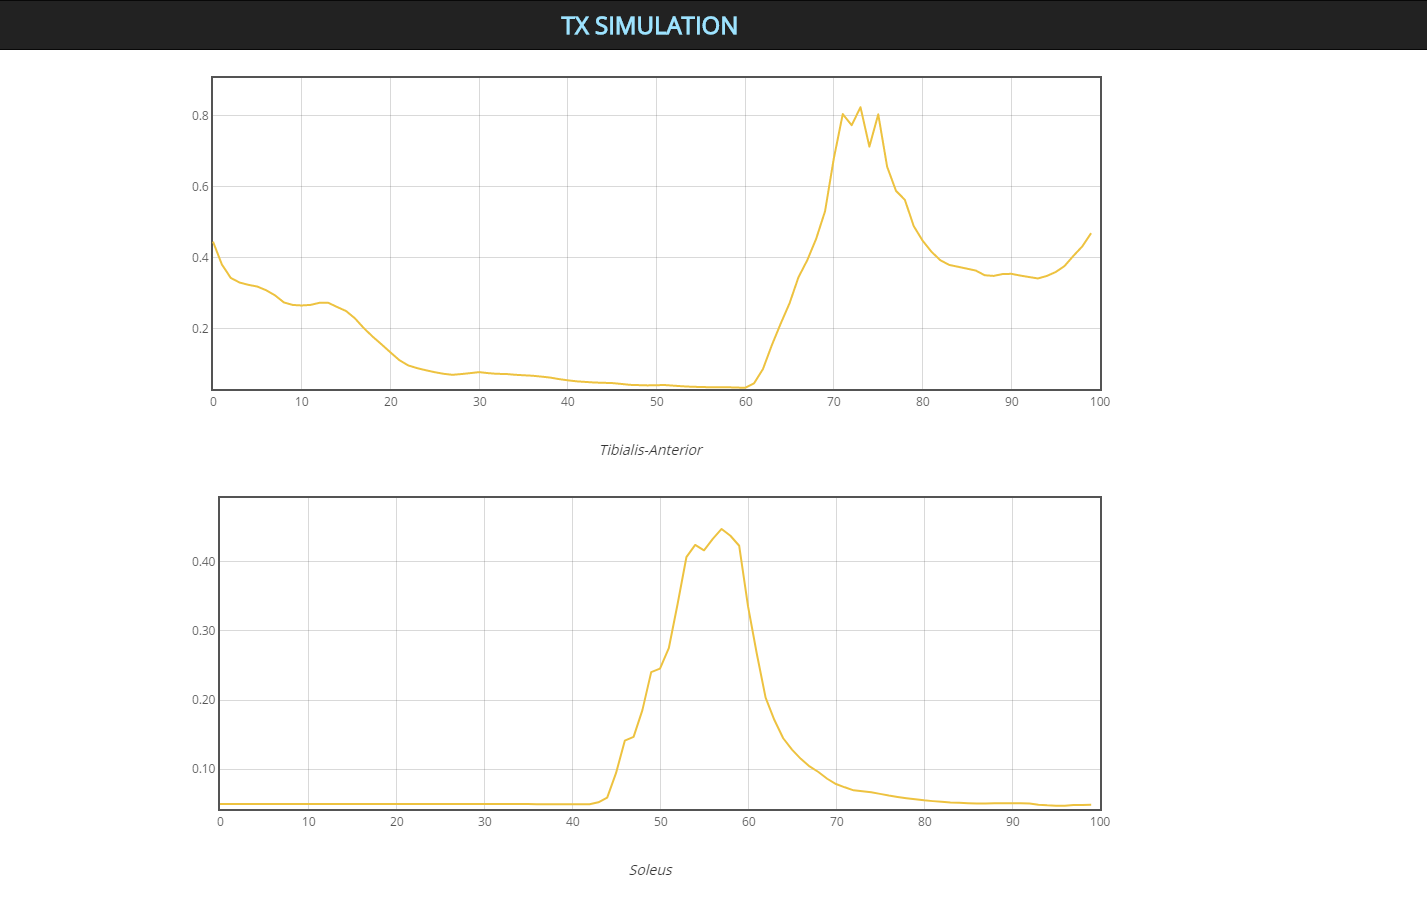
\includegraphics[scale=0.45]{webUI.PNG}
	\caption{Screenshot of the charts displayed in the Google Chrome browser}
  \label{fig:webUI}
\end{figure}
\section{Performance and scalability benchmarks}
In order to test the performance of the model, I have used Virtual Private Servers (VPS) from Digital Ocean. Both MotorSystems had their own nodes with 4 cores, 8GB of RAM and an SSD drive. The Master actor and the Play framework server were on a 2-core node with 2GB of RAM and an SSD drive. The nodes were connected via a private network. 
\\\\
The model was modified so that every MotorSystem had the same number of MotorUnits and so that every MotorUnit was active at every tick. The benchmarks were run for 50 ticks and for each tick, the Master recorded the time it took to complete. The beginning of the tick was the sending of the \textit{ProcessTick} message and the end of the tick was the reception of all \textit{ResultSum} messages from all MotorSystems.
\\\\
The JVM parameters were \textbf{-XX:+UseG1GC} (use the G1 garbage collector) and \textbf{-Xmx6g} for MotorSystems (6GB maximum heap size).
\\\\
The first test consisted in comparing distributed vs. single-node performances. When testing the single-node performance, both MotorSystems were on the same node (with 8GB of RAM) and not on separate ones. The maximum heap size per JVM was lowered to 3GB as both could not have 6GB on an 8GB node. Two tests were performed: one with both systems having 200 MotorUnits and another one with both systems having 400. The figure~\ref{fig:benchmark1} shows all data points generated during the test:
\begin{figure}[H]
  \hspace*{-4cm}
  \includegraphics[scale=0.35]{benchmark1-BIG-2.png}
  \caption{Performance benchmark}
  \label{fig:benchmark1}
\end{figure}
The median tick time values for the 200 MotorUnit test are 10.955s for the single-node benchmark and 5.740s for the distributed one. For the 400 MotorUnit test, the median tick times are 27.876s and 11.549s respectively.  It is clear that the model runs much faster in a distributed fashion.
\\\\
The second test consisted in adding more and more MotorUnits to both MotorSystems running on different nodes to test the scalability of the implementation. Here is the resulting graph showing the result of the benchmark with the maximum number of MotorUnits under 800:
\begin{figure}[H]
  \hspace*{-3cm}
  \includegraphics[scale=0.35]{benchmark2-BIG-2.png}
  \caption{Scalability benchmark, under 800 MotorUnits per MotorSystem}
  \label{fig:benchmark2}
\end{figure}
The model clearly scales linearly. However, with only two nodes and 8GB of RAM per node, the model starts to lag after approximately 800 MotorUnits per system:
\begin{figure}[H]
  \hspace*{-3cm}
  \includegraphics[scale=0.35]{benchmark2-exp-BIG-2.png}
  \caption{Scalability benchmark, more than 800 MotorUnits per MotorSystem}
  \label{fig:benchmark2-exp}
\end{figure}
After 800 MotorUnits, the scalability starts to degrade and becomes exponential. After an investigation, I found out that it was due to memory limits on the nodes: with more than 800 MotorUnits, the heap started to hit the 6GB limit thus triggering full GC at every tick. Full GC is extremely lengthy and it is a 'stop-the-world' operation so it is slowing down the whole simulation very significantly. The solutions for this problem can be:
\begin{itemize}
\item Get nodes with more RAM and increase the heap size
\item Fine-tune the garbage collection for low-pause
\item Try to optimize the code even more to limit the number of allocations
\item Get more nodes
\end{itemize}

\section{Difficulties and problems}
While working on the project, I have encountered several technical challenges:
\begin{itemize}
\item The first challenge was to learn, configure and use Akka. I have never worked with frameworks based on the actor model before so I had to learn the concepts in order to use them. Akka is really powerful and has a lot of features so it was not obvious from the start which ones to use. Moreover, the configuration of Akka Remoting/Clustering and Play can be tedious, especially for things like serialization or cluster configuration. I have also decided to use the Kryo serializer instead of the default Java serializer for inter-JVM communication, as it is much faster. This required even more configuration efforts.
\item Before implementing the web-based UI, I have tried to use ScalaFX, a Scala wrapper around the JavaFX library which used for creating user interfaces for Java applications. It has not proved to be successful as ScalaFX/JavaFX operations are always executed in a single dedicated thread whereas Akka is multi-threaded by design. The problem consisted in creating a communication mechanism between Akka threads and the ScalaFX thread. There is no standard way of achieving this and most of the solutions were quite elaborate. I have then chosen to go with the Play framework/WebSocket solution as it was easier to implement and also provided cross-platform compatibility (the web UI can be displayed from any OS) and thin-client architecture benefits.
\item Another problem was with optimizing the model. I have tried to improve both the time and the memory complexity. The algorithms were not very complicated, so the time complexity was not hard to optimize. However, the memory complexity was a bit trickier to improve. In Scala, immutable structures are the main type of data structures so it was important to make sure to use appropriate data structures (mutable when needed), especially in loops, so as to avoid unnecessary allocations. I have also analysed the execution of the model using a JVM profiler (JProfiler) so as to find the hot spots and the bottlenecks and subsequently remove them.
\end{itemize}

\section{Conclusion}
To conclude, this project has helped me to learn a lot about distributed programming: I have previously used Apache Spark which is completely data-parallel so it was interesting to discover another paradigm and explore the actor model/task-parallel programming. Technology-wise, I have also discovered the usefulness of WebSockets, learned CoffeeScript, discovered the Play framework and also strengthened my knowledge of Scala and the JVM. Finally, I saw the importance of spending time on choosing the right tool for the job: too often engineers would choose a technology because of its hype factor or because of its reputation, not because of its actual suitability for the problem. I saw once again, that using a technology that is fit for the problem is crucial for achieving an effective and an appropriate solution. 

\end{document}
